\section{Implementation of Scratch Detector}
In this chapter the development and results of a YOLOv5 solution for detection of scratches found on printed layers of a 3D binder jet printer. The following subsections will extend and go in-depth on the list of challenges presented in TODO and present solutions and ideas to handle them.

\subsection{Labeling the Dataset}
TODO: verallgemeinern mit scratches \\

\textbf{The first challenge:}
As mentioned \ref{intro:challenges}, some scratches are weaker and should not be marked as actual scratches to not make the model too sensitive. A sensitive model would lead to many false positive detections like a thicker edge or an oxidation spot. The main goal would be to find a metric that can evaluate the prominence of the scratches. With such a metric, each annotated scratch will have a prominence value and therefore a minimum threshold could be used to eliminate the weaker scratches.

\textbf{The solution:}
A proper metric should measure how dark a scratch line is with respect to it's neighboring background. Also, the metric should not take in consideration the length or width of the scratch.
The metric developed for this project works as follows:
Crop the bounding box from the image. Because the image is a grayscale, the cropped image will have only 1 channel i.e. it can be interpreted as a 2D array. The rows of the array are normalized and the mean row is then calculated. For clarification: the mean row is obtained by summing all rows into 1 row and dividing each element of that row by the total number of rows. The center values of the mean row are usually lower than the values from the start or end of the mean row, because the bounding box has the scratch with darker pixels positioned in the center. The plot of the mean row would look like the hyperbole of $f(x)=x^2$. The mean row is then multiplied by -1 and the plot would look more similar to $f(x)=-x^2$. This mean row multiplied by -1 can be interpreted as single pulse of a signal and the prominence of this signal pulse can be calculated by using special signal processing functions like TODO. \\
TODO figure of metric here. \\

Darker scratches will tend to have a higher prominence value than the faded ones. Now the only thing left to do is to choose a threshold and filter out the weak scratches. \\
During the filtering process, it was obeserved that some scratches had a surprisingly low prominence value. Usually, this was because the bounding box was not properly sized and the edges of a printed part were contained. Because the edges are dark, this would make the signal curve flatter and therefore the prominence value would be smaller. A resizing or centering of the bounding box solved this problem.

TOOD figure of bb with edges here. \\


\subsection{Bitmask Integration}

\textbf{The challenge:}
As discussed in TODO, the images of the layers have two types of anomalies:
\begin{enumerate}
\item thick edges or closely positioned segments that look like scratches
\item artifacts from previous layer that look like scratches
\end{enumerate}

This situations might trick even humans and during labeling it was found out that each potential scratch had to be checked by looking the current bitmask and the previous bitmask. The current bitmask was used to check against the first type of anomalies and the previous one for the second type of anomalies. This lead to the intuition of integrating the bitmasks in the training process.
 However, most object detectors take as input exactly one image with the respective annotations. The challenge is to find a proper way to integrate the two bitmasks with each image and provide the model this extra context information.


\begin{figure}[ht]
  \centering

  \begin{subfigure}{0.75\textwidth}
    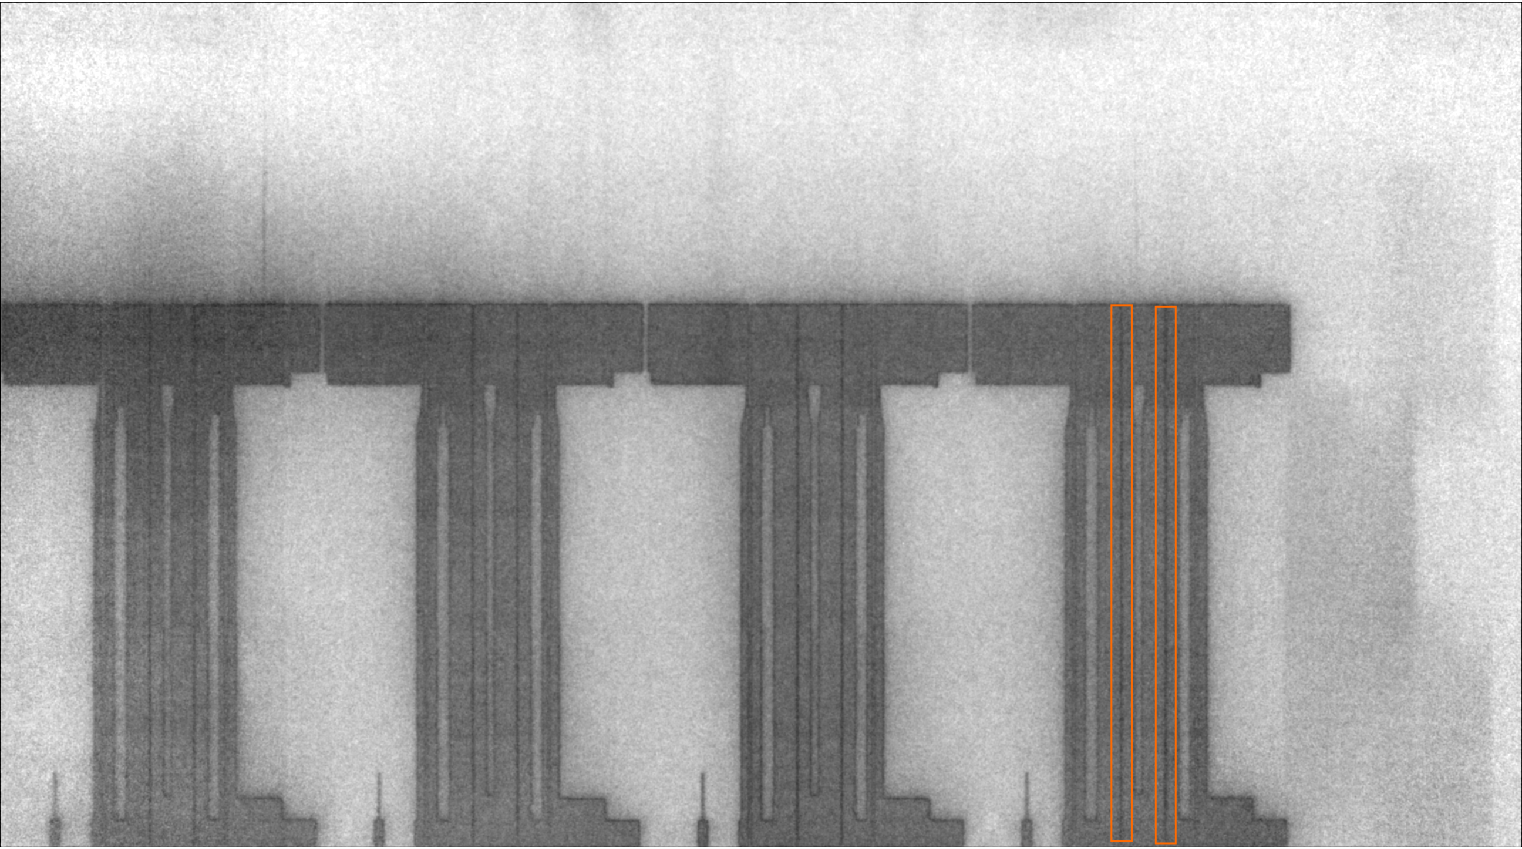
\includegraphics[width=\textwidth]{images/layer_01486_marked}
    \caption{Layer with thin splits marked in orange bounding boxes.}

  \end{subfigure}

  \begin{subfigure}{0.75\textwidth}
    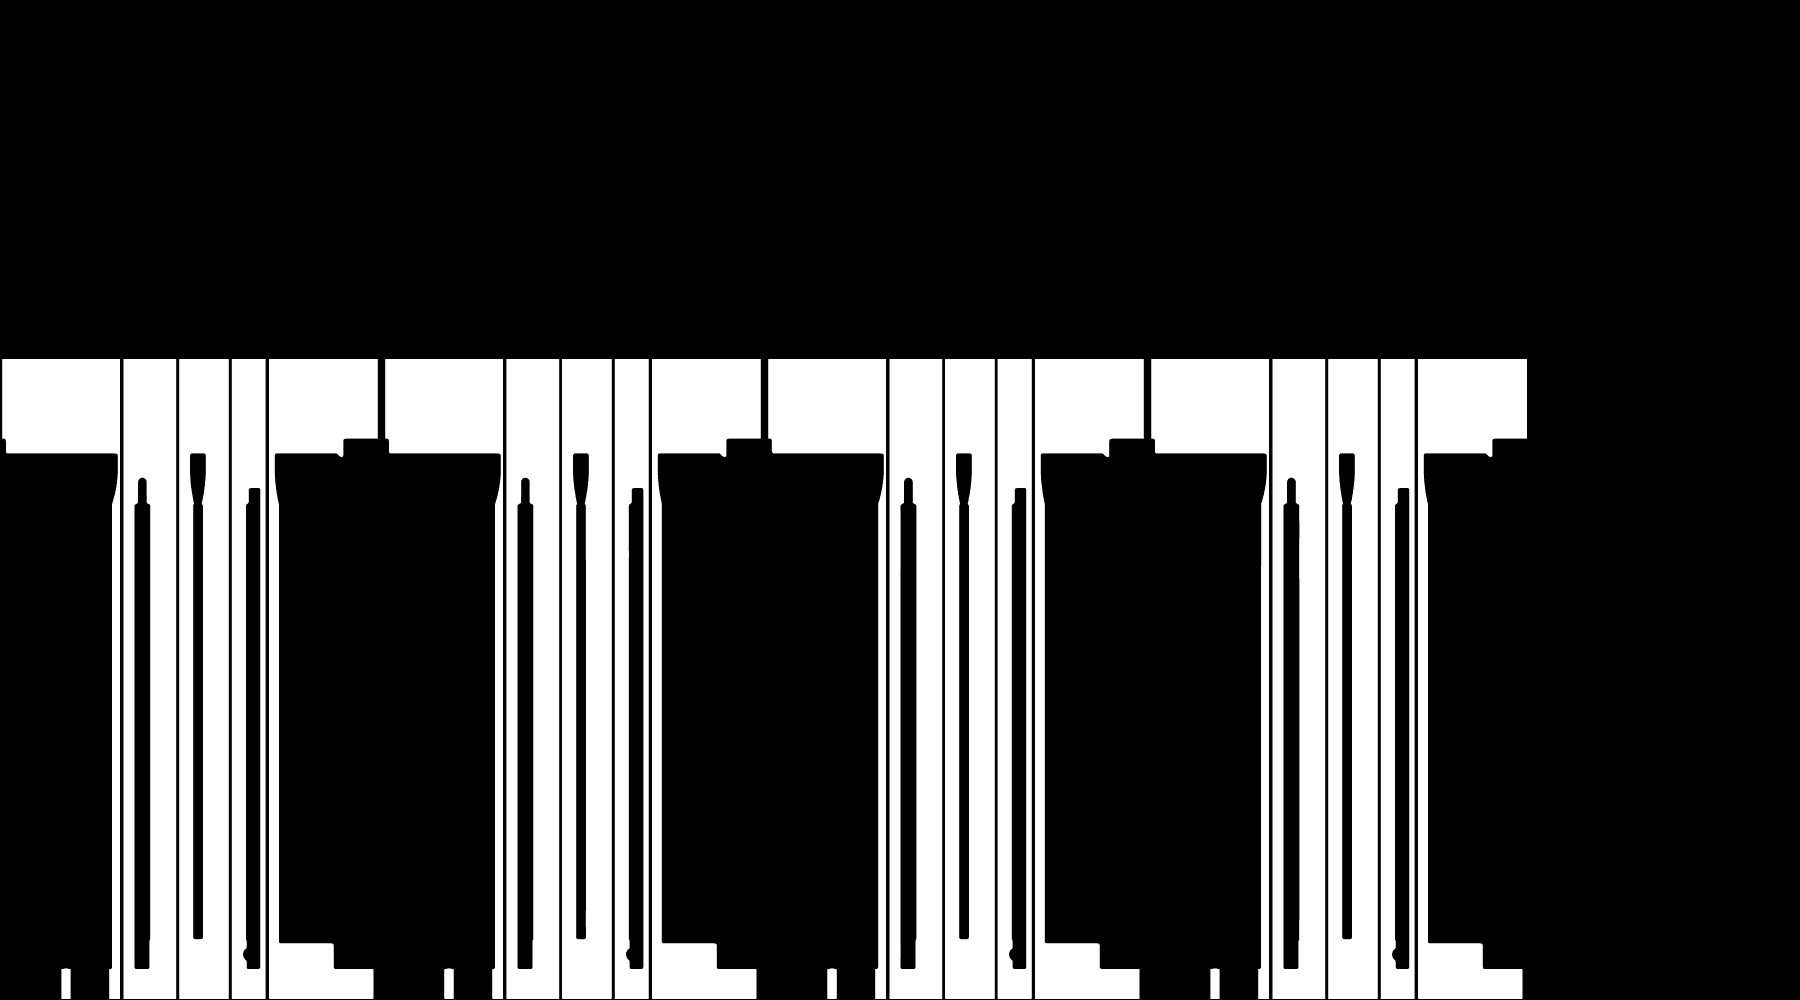
\includegraphics[width=\textwidth]{images/bitmask_01486}
    \caption{Corresponding bitmask must be checked to see if it's a scratch or a thin split.}
  \end{subfigure}

  \caption{Thin splits. TODO horizontal allign, better images}
  \label{fig:thin_splits}

\end{figure}

\textbf{The solution:}
YOLOv5 works with RGB images and if a grayscale input image is detected, it gets converted to RGB. This conversion provides no extra information and is more a preprocessing step. An alternative conversion method is to represent the grayscale with a single channel only e.g. the red one and the other two channels are just some blank images. \\

TODO figure with the conversion methods. \\

The second conversion methods will free up two channels that can be used to add relevant context information. With the challenge statement in mind, filling up the other two channels with the current and previous bitmasks is clearly helpful e.g. the green channel contains now the current bitmask and the blue channel contains now the previous bitmask. This is possible, because the bitmask images are also grayscale images. So instead of providing a grayscale image as an RGB image, three grayscale images are provided as an RGB image. \\

TODO figure to show new image mode \\

This new type of input image proved to make the model more robust against the above described anomalies, but with this new input some consideration and adaptations need to be made. \\
The layer images and the bitmask images have the same ratio, but different sizes of respectively 2592x1440 and 1800x1000. On one hand, the layer images can be downscaled to 1800x1000 and some image information is lost. On the other hand, the bitmask can be upscaled and the pixel-perfect edges get blurred. Another approach would be to meet somewhere in between e.g. downscale the layer images to 2196x1220 and upscale the bitmasks to 2196x1220. This trade off can be however avoided, if the the bitmasks are upscaled to the resolution of the layer images and a threshold on pixel values is used i.e. the pixels with a value below 0.5 are set to 0 and the rest are set to 1. The upscaled and thresholded bitmasks will retain this way all the pixel precise context information.  \\
Now the inference step will also need an extra pre-processing step to include the bitmasks and without them the inference is invalid. Also, the first layer is a special case, because it does not have a previous bitmask and the current layer is inserted twice. \\
This concept of filling the channels with context information was tested under many variations, but the one presented above delivered the best result. Most variations kept the original input image as the first channel and used different ways to fill up the other two channels. Some example of variations are:
\begin{itemize}
\item layer image and twice the current bitmask
\item layer image,the current bitmask and a logical OR of the current and previous bitmasks
\item layer image, the current Sobel-filtered bitmask and the previous bitmask
\end{itemize}
The first example does not include any information about the previous bitmask, so the second type of anomalies, the artifacts from previous layers, are detected as edges. The second example was problematic in some cases, because a logical OR of two bitmasks might treat a gap between two segments from the previous layer as a printed region. This leads to detecting a thin gap as a scratch. In the third example the initial intuition was that a Sobel-filter will directly show where the edges are, but the problem is that information about the current printed regions is lost. The list of variations is long, but those were some examples to get an intuition how context information is lost or malformed.

\subsection{Windowing}

\textbf{The challenges:} In the current release of YOLOv5 rectangular images are not that well supported. Data shuffling during training is available only for square input images, which is needed for a more robust training. Internally, rectangular images are actually padded to a square shape. This means that the images can be simply padded before using them as input to YOLOv5, but is the color or method of padding relevant? If so, how does this affect the training? \\
Another problem during development are questionable scratches like the ones that are positioned exactly on the edge and weird regions like oxidation spots. The easy way would be to simply ignore those images, but what if the image contains only one questionable scratch and three prominent scratches? The luxury of throwing away images is not very affordable with this small dataset. Remember that the dataset on hand is minuscule in comparison with open datasets. \\

TODO maybe show questionable scratches and oxidation spots \\

The current images have a resolution way bigger than the average open datasets, so smaller batch sizes and/or longer training times are to be expected. Is there a way to use as training input only relevant regions of the images without losing any performance?\\

\textbf{The concept solution:} All the above problems can be solved by dividing the input image into smaller windows and training the model on those windows, called "windowing" for short.  However, there are many variables and considerations to be made:
\begin{itemize}
\item What is the optimal window size?
\item Is an overlap between the windows needed?
\item Are there any problems, if a scratch is not completely contained in a window?
\item What are the windowing strategies?
\item How to identify relevant windows?
\item How is the inference impacted?
\end{itemize}
The multiple sub-challenges together with those additional considerations make the topic of windowing more complex, but during this section an in-depth analysis of the windowing process will be made.

\subsubsection{Window Shape and Size}
As stated in the challenges, YOLOv5 is designed to work with square images. Using rectangular images disables data shuffling during and training and adds more potential side-effects with the padding of rectangular images to square images. The padding can have a color like the mean image color, or it can be a reflection of the last pixels. All those problem simply disappear, if the input image is subdivided into equally sized square windows. If needed, the neighboring windows might have an overlap to be able to use any desired window square size. TODO explain overlap better \\
There are two types of images with respect to the count of annotations: normal images that have at least one annotation and background images that have no annotations. Because of the windowing, the number of background images can be quite large, but for the moment it is safe to not use them for training, because the official YOLOv5 documentations recommends a range of 0-20\% of the training dataset to be background images. \\
The next step is to take the right square size. Smaller windows will decrease the training time, and the questionable scratches and weird regions can be easily filtered out from training. The downside is that some scratches might get split into multiple windows and in some cases the splits are very unlucky e.g. one window might contains only 5\% of the original scratch. With bigger windows, the problems and benefits go in the opposite directions: the granular control of the scratch and region filter is lost, the training times increase, but the scratch splitting problem is less prevalent. The only constraint imposed by YOLOv5 is that windows width and length need to be a multiple of 32.\\

TODO make this table \\
228 layers \\
ds : train s, val s, inf s, inf im count, gen time PE 300 layers \\
1280 : 93 s, 9 s, 82 s, 1368 im, 11 s \\
960 : 36 s, 4 s, 47 s, 1368 im, 11 s \\
640 : 32 s, 3 s, 67 s, 3420 im, 10 s \\
320 : 14 s, 2 s, 105 s, 10260 im, 10 s \\

In set of tests the smallest window size was 320x320 and the size was increased then by 320 after each test. The final window size was 1280x1280. As it can be seen in table TODO, the bigger window sizes provided the best mAP at the cost of higher training times. One surprising fact was that the 1280x1280 windows provided a stable and robust training, despite the fact that bigger windows are more likely to contain unwanted regions. This situations were actually rare, because the questionable scratches and weird regions were usually situated very far from the good scratches. This is a bit of a lucky situation. \\
The avoidance of scratch splitting was somewhat helpful when training with bigger windows, but it seemed unlikely that this was the only contributing factor for better metrics, since scratch splitting occurred on less than 5\% of the total scratches. Also, the edge cases, in which the smaller split of scratch was below a threshold length, was filtered from the dataset.  \\
 A hypothesis is that larger windows provide more examples of scratch-free printed parts, which might contain some interesting cases like a darker edge or a gradient of gray. This in turn makes the model more robust. An initial naive approach was to put more background images in the 640x640 dataset, but the problem is that it even with the higher bound of 20\% background images it did not work. This is because many of the background images were irrelevant and did not contain printed parts. A second approach was to split each window of the 1280x1280 datasets into 4 640x640 windows. With this second approach, "double windowing", the results were similar to the experiment with 1280x1280 windows! TODO say where to see this in the table. The batch size on the double windowed dataset can be increased about 4 times, which leads to better batch normalization. \\

TODO example of background vs double windowing \\

Another interesting discovery is that it's better to split the dataset after the windowing has been done. This ensures a more similar distribution between the splits. This observation alone stabilized the training experiments very much. \\




\subsubsection{Windowing Strategies}
In the subsection from above a "grid windowing" strategy was assumed and as the name suggests, the corners of a grid are used to determine how to extract the windows. In a more advanced form, grid windowing also overlaps the neighboring windows. This helps avoiding the extreme cases of scratch splitting as seen in figure TODO. One problem with grid windowing is that some layer are very similar to each other and also repeat the scratches at the exact same locations. This makes many windows to be repetitive.\\
A second window strategy, "random windowing", each scratch is initially contained in a window. The windows are then shifted randomly along the X and Y axis. This avoid the problem of repetitive windows described in grid windowing. \\
In multiple head-to-head comparison the 2 strategies traded victories. One important remark is that the grid windowing strategy was actually very stable and the metrics barely fluctuated. This is because the actual windows never change. Meanwhile, the random windowing strategy fluctuates about 7\% from the average metric baseline. This is mostly, because the randomness can be sometimes very unlucky and for example split multiple scratches. \\

TODO insert image here \\

\subsubsection{Adaptations for Detection}
If a model is trained on windows instead of the original images, some pre- and post-processing steps for detection need to be considered. \\
Before the detection, images need to be split in windows of similar shapes used in training. The strategy needs to be grid windowing, because all areas of the images need to be detected and this strategy makes reconstruction of the image easier. Also, an extra set of window between neighboring windows can be used to avoid scratch splitting. TODO ex image cu asta. \\
After the detection, the windows with the respective detections need to be reconstructed to the original window. One naive way would be to draw detections on the windows and the reconstruct the windows into the original image. However, the trick is that with grid windowing every window has a predetermined position and the actual reconstruction of a new image can be avoided. In this implementation of grid windowing, the position of a window is specified by the upper left corner, width and height. This meta information can be easily encoded e.g. in the name of the file. Let's assume that a window of size 640x640 extracted from the corner TODO, TODO contains a detection. This detection can now be translated by TODO, TODO pixels and a valid detection for the original image is obtained. The translated detections can now be drawn directly in the original image.\\
 Note that the detection is in YOLO format and the position of the initial detection is expressed in normalized coordinates with respect to the window size.Therefore, a conversion of the detection from the YOLO label format to COCO format (TODO ref for formats) for the translation step is needed. After the translation, the detection can be converted back into the YOLO format.  Alternatively, the translation can be normalized with respect to the original image size.\\
 The naive way is at least 10 times slower, but it still was able to deliver a few FPS, which for this project is actually acceptable. A real-time detection is however possible with the second approach. \\
 Another post-processing step after the translation of the detections is the merging of detections. Because scratches might get split, the respective detections should be some overlapping bounding boxes. Those bounding boxes need to be also merged. The problem is that sometimes the bounding boxes might no overlap at all and be even a few pixels apart and that is why an extra set of windows as shown in TODO is used. This helps in connecting the disjointed detections. \\



\subsection{Augmentations}
The dataset at hand features a total of 2295 images of layers with the corresponding bitmask, but only a fraction of the images contain an actual scratch. This is far from the recommended minimum of 1500 images per class and 10000 instances per class. \\
It is important to make distinction between online and offline augmentations. With offline augmentations the images are augmented before the training and with online augmentation the images are augmented every epoch during the training. With a relatively small increase of training time, online augmentation provide a more robust training with the extra variance in the dataset, but sadly, not all augmentations methods can be implemented as online methods due to some technical constraints imposed by albumentations, the augmentation library used internally by YOLOv5 and YOLOv5 itself. The first constraint is that every augmentation method can have as input exactly one image with a list of bounding boxes. The second constraint is that the output is exactly one image with a list of bounding boxes. The third constraint is that the input image size needs to correspond with the output image size. \\
Basic augmentations methods like contrast and brightness manipulations are not affected by those constraint, but the random windowing is affected by this. Technically speaking, the random windowing is not an augmentation step, but it would be nice to be able to provide during each new epoch a new randomly shifted window for all scratches. This alone might stabilize the whole method and not face the fluctuations as discussed in TODO. TODO this some relevant future work, online random windowing if implemented like mosaic and cut-mix.\\
Among the online augmentations, there is a special group that are able to circumvent some of the constraint. Those are some online augmentations that come out-of-the-box with YOLOv5 like CutMix and Mosaic. \\

\textbf{Mosaic:} The mosaic augmentation is an online augmentation that takes 4 images and combines them into 1 image. This augmentation is built-in the YOLOv5 project and the constraint regarding the input for online augmentations is circumvented.
The input images are also downscaled at different rates, which helps increase the variance . A trade-off is that the new image actually contains smaller scratches, which raises the question if this has an positive or negative impact. This question is discussed in-depth in the paragraph about the stretch augmentations. \\
The parameters for this augmentation are only the probability of it being applies. The downscaling factors of the images, the number of the input images and the pick distribution are not parameterized. TODO future work improved mosaic paper https://iopscience.iop.org/article/10.1088/1742-6596/1684/1/012094/pdf
Because of this unidimensional parametrization, the experiments were simply testing the effects of the mosaic augmentation at increments of 0.1 for the application probability. The results favored a application probability range between 0.5 and 0.8. This upper bound of 0.8 is a first indicator that the shrinking of the scratches might be problematic. Note that for higher application probabilities the results were actually ok e.g. the mAP@0.5 was only about 2\% smaller on average. The slightly more visible aspect was that for higher probabilities the bounding boxes were on average shorter, but still able to have an  IoU greater than 0.5. \\

TODO example image mosaic

\textbf{Cut-Mix:}
The cut-mix is sometimes seen as mosaic augmentation with only 2 input images, but an important distinction needs to be made. The cut-mix crops a regions from an image and pastes it over the other input image at a random location. This was problematic, because sometimes the cropped region was partially or completely covering a scratch. The complet covering of a scratch is simply unwanted information loss and the partial covering was worse than the split scratches, because there is no way of filtering tiny splits like in the windowing process. \\
As before, the only parameter available is the application probability. Sadly, there is no way optimize/avoid the covering of scratches with the cropped image. For this reason this augmentation method was not used. \\
TODO future work improve this with control over filter small scratch splits or position of the pasted region
TODO example image of problem with covering


\textbf{Translate and Scale: }
Those two online affine augmentations are ok, if used carefully. Like before, they have only one parameter, but this time the parameter specifies the translation or scaling range e.g. 0.5 specifies a range of -0.5 to 0.5. For small ranges of up to +/- 0.2 for the translation and up to +/- 0.3 for the scaling the model trains with a nicely varied data. For higher ranges each augmentation had it's own problems. The translation moves the location of the scratch around, but image data is traded for black pixels like in figure TODO. This reduces the amount of relevant background information that provide counter-examples for scratches e.g. thick edges. The scaling affects the average width of the scratch, which in the datasets barely varies by a few pixels. \\

TODO figure cu translation care pierde thick edge \\

TODO future work improve translation \\


\textbf{Stretch and Squeeze:}
YOLO detectors usually have some hyperparameters the bounding boxes called anchors. The anchors are used as prior by the model for the location and shape of the bounding boxes. Ideally, before every training experiment the anchors need to be optimized with respect to the dataset. For newer YOLO versions this done automatically. With the help of windowing and translations the datasets contains a good variance for the positions of the bounding box and also the width barely varies. However, the length varies from 30 pixels to even above 600 pixels. Also, augmentations methods like mosaic tend to shrink the scratches and windowing introduces split scratches. This makes the training biased towards shorter scratches and the performance on longer scratches might be suboptimal. \\

TODO plot distribution \\

In order to test the hypothesis, if shorter scratches make the detection of longer scratches worse and vice-versa, an artificial dataset was used. Images were generated by drawing thin and long rectangles on a white background. For testing the hypothesis three artificial datasets, \textit{short scratches}, \textit{medium scratches}, and \textit{long scratches}, were generated. Then, the model was trained on those datasets, generating the corresponding weights \textit{short weights}, \textit{medium weights}, and \textit{long weights}. Each of the weights was then used for detections on each test split of the three artificial datasets. The results are seen in table TODO and it can be seen that YOLOv5 is more robust on detecting scratches from \textit{short scratches} dataset with the weights \textit{long weights}, than vice-versa, detecting on \textit{long scratches} with \textit{short weights}. Because the artificial dataset contains trivial examples, almost all the scratches were detected and the errors were mostly localization errors i.e. IoU below the 0.5 threshold. The IoU threshold can be lowered to 0.35, since a general localization is for this project good enough, but the problem of localization becomes a bit more serious, if the datasets images are split into windows. This is because the localization errors occur because the detected bounding boxes are shorter than the ground truth bounding boxes and for windowing this means that in some cases the detected bounding boxes might not overlap for neighboring windows, which leads to two small double detections in the original image. Therefore, there is a need to provide somehow longer scratches. The initial thought might be to use the scaling augmentation methods, but the method cannot be set to only scale larger and also the width of the scratch might be altered. \\
An alternative approach is to stretch the scratches by deleting a few upper or lower rows from the image and then resizing the image back to the initial size. This keeps the width unaltered. This stretch augmentation method is then used on the \textit{short scratches} dataset and it can be seen that the results on detecting \textit{long scratches} is improved. \\
This augmentation method needs to be augmented as a custom online augmentation method in YOLOv5. The current implementation uses only one factor that specifies at what rate the length of the image is reduced before stretching it back to the initial shape. \\
The other way around is to use a squeeze augmentation method and this works by using windows that are randomly taller than the desired window height, then the windows are resized to the desired window height. This method is not possible to implement as an online augmentation method, because the taller windows cannot be squeezed due to the constraint of equal input and output size. Another approach might be to retrieve some corresponding upper or lower image rows of the respective window, but this is not possible, because the name/id of the window is not known. Therefore, this can be technically implemented as an offline augmentation methods. \\

TODO table short, medium, long, stretched


\textbf{Constrast:} As stated in TODO, scratches might be more or less prominent, but this effect can be in a way simulated with contrast changes. This method can be implemented as a custom online augmentation. The current implementation uses one parameter for the application probability and one parameter for the range of the contrast change. \\
In most experiments a contrast change of +/- 0.15 with any application probability helped the model be more robust and less false positive were detected. \\

\textbf{To avoid:}
hsv
occlusions:
  - random erase, cutout not working
  - similar effect scratch splitting
brightness

mixup not workingF



\subsection{Hyperparameter Optimizations}

\textbf{Model Size}

\textbf{Hyperparameter evolution}

\textbf{Batch Size}
The official documentation recommends that training should be performed on the biggest batch size possible in order to produce the best batch normalization statistics, but meanwhile on the official Github repository the developers suggest that YOLOv5 is batch agnostic (TODO source). For the sake of finding the truth, multiple experiments with varying batch sizes have been made. The results were that for batch sizes up to 64 the map@0.5:0.95 metric was in favour of bigger batch sizes. Other metrics had no tangible differences. Bigger batches required more than 2 GPUs or compromising to a smaller window size. \\
TODO show results \\

\textbf{Learning Rate and Gradient}
The initial experiments showed high jumps after each epoch, so a switch from the standard stochastic gradient descent to AdamW has been made. The documentation recommends for AdamW to change the learning rate from 0.01 to 0.001, but a step size of 0.0001 showed a more stable evolution from epoch to epoch.
TODO maybe show some results

\textbf{Loss Function}


\textbf{IoU threshold}


TODO obiective dataset:
scratches position
scratches length should have variety (prin stretch si prin window cuts)
scratch strength variety (sa inventez ceva)

easy source code modifications (la metrics mai ales)
dataset format
dataset postprocessing (black border)



\subsection{Development Environment \& Setup}
TODO draft available, write it at the end

Bounding Box Debugger
